Otrzymane dane były podzielone na dwa zbiory: testowy (400 przykładów) i uczący (100 przykładów) (Tab. \ref{tab:count}). Dane posiadają cztery zmienne ($x_1, x_2, x_3, x_4$, jednak ze względu na wysoką korelacją (bliską jedności) pomiędzy $x_1$ i $x_3$ (Tab. \ref{tab:corr}), tylko jedna z nich będzie najprawdopodobniej analizowana w kolejnych etapach.
    \begin{table}[h]
    \begin{center}
\begin{tabular}{|c|c|c|}
\hline
                                    & klasa 1 (zielony)                  & klasa 2 (czerwony)\\ \hline
zbiór uczący                        & 27                       & 73      \\ \hline
\multicolumn{1}{|c|}{zbiór testowy} & \multicolumn{1}{c|}{145} & 255     \\ \hline
\end{tabular}

\captionof{Tab. 1 }{Liczebność zbiorów i klas.} \label{tab:count}
\end{center}

\end{table}
\begin{table}[h]
\begin{center}
\begin{tabular}{|c|c|c|c|}
\hline
\multicolumn{1}{|c|}{}   & \multicolumn{1}{c|}{$x_1$}                       &  $x_2$                       & $x_3$                       \\ \hline
\multicolumn{1}{|c|}{$x_1$} & \multicolumn{1}{c|}{\cellcolor[HTML]{C0C0C0}} & \cellcolor[HTML]{C0C0C0} & \cellcolor[HTML]{C0C0C0} \\ \hline
$x_2$                      & 0,0117                                        & \cellcolor[HTML]{C0C0C0} & \cellcolor[HTML]{C0C0C0} \\ \hline
$x_3 $                      & 0,9969                                        & 0.0101                   & \cellcolor[HTML]{C0C0C0} \\ \hline
$x_4$                      & -0,2117                                       & -0,0808                  & -0,2109                  \\ \hline
\end{tabular}

 \captionof{Tab. 2 }{Korelacja pomiędzy zmiennymi dla danych uczących.} \label{tab:corr}
 \end{center}
\end{table}



\begin{figure}
\centering
\begin{subfigure}{.5\textwidth}
  \centering
  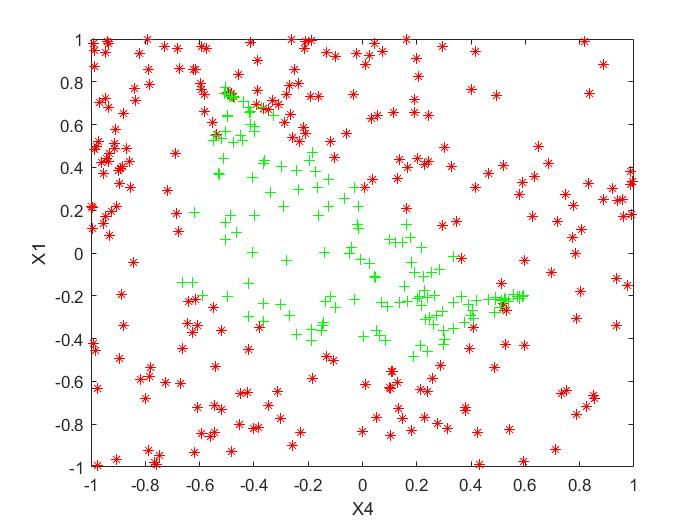
\includegraphics[width=\linewidth]{assets/test.jpg}
  \caption{Zbiór testowy}
  \label{fig:sub1}
\end{subfigure}%
\begin{subfigure}{.5\textwidth}
  \centering
  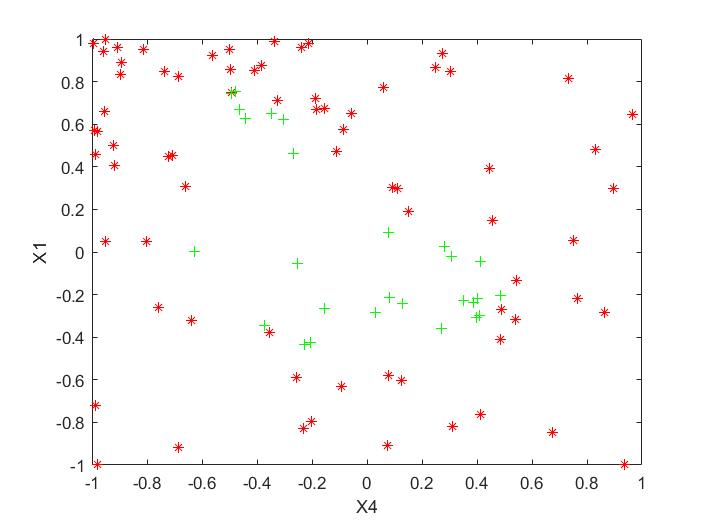
\includegraphics[width=\linewidth]{assets/train.jpg}
  \caption{Zbiór uczący}
  \label{fig:sub2}
\end{subfigure}
\captionof{Rys. 1}{Wizualizacja danych}
\label{fig:test}
\end{figure}
\FloatBarrier
Klasy nie są liniowo separowalne, ale 
rozłączne. Na danych wykonano operacje normalizacji i centralizacji,
Czy klasy mają części wspólne?
• Jaka powinna być minimalna liczba neuronów
ukrytych do wykonania zadania klasyfikacji i
dlaczego?